
\section{Multi-Bit Modulatoren}

Anstatt eines Komparators ADCs mit mehreren Bits für den Aufbau des Sigma-Delta-\textbf{Modulators} verwendet.

\begin{minipage}[t]{0.48\columnwidth}
    \begin{itemize}
        \item[+] \textbf{Dynamikgewinn von ca. $\bm{6 \, \deci \bel }$ pro zusätzlichem Bit.}
    \end{itemize}
\end{minipage}
\hfill
\begin{minipage}[t]{0.48\columnwidth}
    \raggedright%
    \begin{itemize}
        \item[-] Aufwändiger Flash-ADC (parallele Komparatoren) nötig, da in einem Takt gewandelt werden muss
    \end{itemize}
\end{minipage}


% weglassen? von Slides abgeschrieben...
\subsection{1 Bit vs. Multi-Bit ADC (im Modulator)}

\begin{itemize}
    \item ADC ist unproblematisch, da hinter Integrator (siehe Blockschaltbild Abschnitt~\ref{Aufbau Sigma-Delta-ADC}) und damit 
        Teil vom Quantisierungsfehler
    \item 1-Bit ADC (Komparator) nichtlinear \textrightarrow\ ADC-Verstärkung signalabhängig
    \item Es entsteht ein nichtlineares System
\end{itemize}


% weglassen? von Slides abgeschrieben...
\subsection{1 Bit vs. Multi-Bit DAC (im Modulator)}

\begin{outline}
    \1 DAC muss volle Präzision des (gesamten) Wandlers haben
        \2 DAC-Spannung wird direkt mit Eingangsspannung 'verrechnet'
    \1 1-Bit DAC ist perfekt linear (nur Offset- und Gain-Fehler, welche statisch kompensierbar sind)
    \1 DAC muss sehr genau sein \textrightarrow\ kann kalibriert werden
        \2 Drifttemperatur und Alterung sind dennoch ein Problem
\end{outline}


\subsection{Dynamic Element Matching (DEM), Mismatch-Shaping}

\begin{minipage}[c]{0.4\columnwidth}
    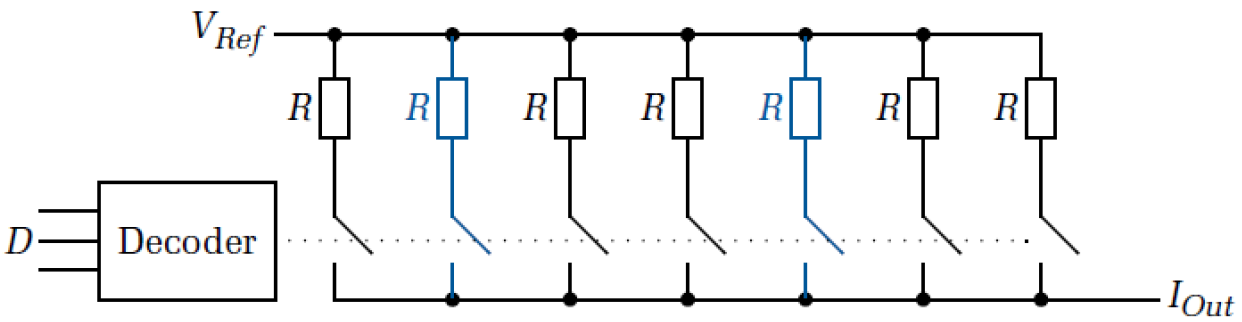
\includegraphics[width=\columnwidth]{images/strom-DAC.png}
\end{minipage}
\hfill
\begin{minipage}[c]{0.58\columnwidth}
    \begin{outline}
        \1 Widerstände des DAC müssen perfekt matchen (so gut wie DAC-Genauigkeit)
            \2 In der Praxis ist das nicht möglich!\\
                \textrightarrow\ mismatch
    \end{outline}
\end{minipage}

\vspace{0.2cm}

\begin{outline}
    \1 Dynamic Element Matching (DEM): Spezieller Algorithmus
        \2 Einschalten der einzelnen Widerstände wird dynamisch umgestaltet, so dass Ausgangskennline des DAC 
            'durchschnittlich linear' \\
            \textrightarrow\ Systematischer Fehler wird in Zufallsfehler (Rauschen) umgewandelt
    \1 Mismatch-Shaping 
        \2 Zufallsfehler (Rauschen) wird mit Noise-Shaping gedämpft
\end{outline}


\subsection{Fazit Sigma-Delta-Modulatoren}

\begin{minipage}[t]{0.48\columnwidth}
    \begin{itemize}
        \item[+] Signal wird nicht (wenig) verändert mit Tiefpass
        \item[+] 1 Bit DAC perfekt linear 
        \item[+] 1. SNR-Erhöhung durch Oversampling ($3 \, \deci \bel$ pro Oktave)
        \item[+] 2. SNR-Erhöhung durch Noise Shaping ($6 \, \deci \bel$ pro Oktave)
        \item[+] 3. SNR-Erhöhung durch ADC/DAC im Modulator ($+6 \, \deci \bel$ pro Bit)
    \end{itemize}
\end{minipage}
\hfill
\begin{minipage}[t]{0.48\columnwidth}
    \begin{itemize}

        \item[+] Modulatoren 1. Ordnung immer stabil ($90 \degree$ Phasenschiebung)
        \item[+] Modulatoren 2. Ordnung meistens stabil
        \item[-] Modulatoren höherer Ordnung können instabil werden  
        \item[-] 1 Bit ADC (Komparator) nichtlinear
        \item[-] \textbf{Pattern Noise} 
    \end{itemize}
\end{minipage}


\subsection{Digitalfilter}

Der digitale Teil des Sigma-Delta-ADCs kann auf mehrere Arten realisiert werden.  Das Digitalfilter soll die folgenden Aufgaben
erfüllen:

\begin{minipage}[t]{0.55\columnwidth}
    \begin{itemize}
        \item Reduktion des Rauschens (wegen Noise-Shaping viel Rauschen bei hohen Frequenzen)
    \end{itemize}
\end{minipage}
\hfill
\begin{minipage}[t]{0.42\columnwidth}
    \begin{itemize}
        \item Erhöhung der Auflösung
        \item Redution der Sample Rate
    \end{itemize}
\end{minipage}


\subsubsection{Mittelwertbildung}

Einfachste Mittelwertbildung umgesetzt mittels countern \textrightarrow\ Funktionsweise und Formel 
siehe Abschnitt~\ref{Sigma-Delta-modulator Ordnung 1}


\subsubsection{Kammfilter (Mittelwertfilter)}

\begin{minipage}[t]{0.45\columnwidth}
    \begin{tabular}{ll}
        $Z^{-1}$    & um $1$ Takt verschieben \\
        $Z^{-L}$    & um $L$ Takte verschieben \\
    \end{tabular}
\end{minipage}
\hfill
\begin{minipage}[t]{0.52\columnwidth}
    \begin{tabular}{ll}
        FIR    & Finite Impulse Response \\
        IIR    & Infinite Impulse Response \\
    \end{tabular}
\end{minipage}

\vspace{0.2cm}

\begin{minipage}[t]{0.58\columnwidth}
    \begin{center}
        \myul{FIR-Filter}
    \end{center}
    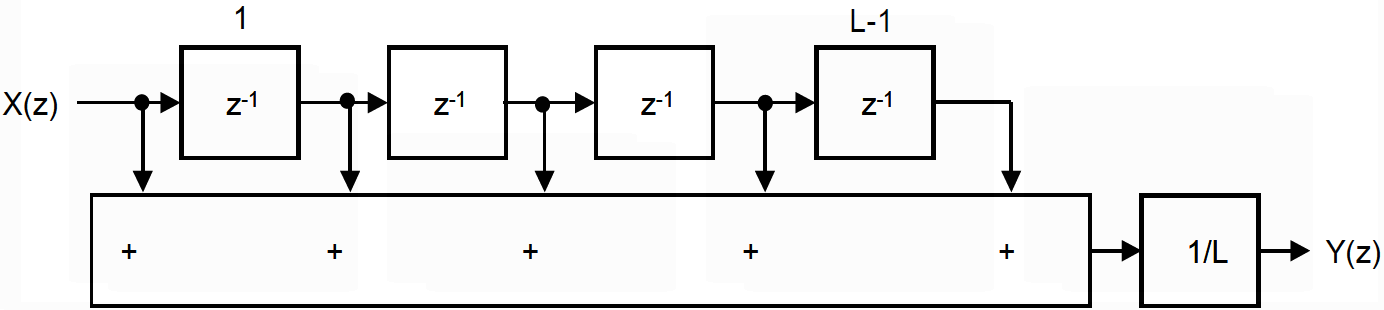
\includegraphics[width=\columnwidth]{images/kammfilter.png}
\end{minipage}
\hfill
\begin{minipage}[t]{0.38\columnwidth}
    \begin{center}
        \myul{IIR-Filter}
    \end{center}
    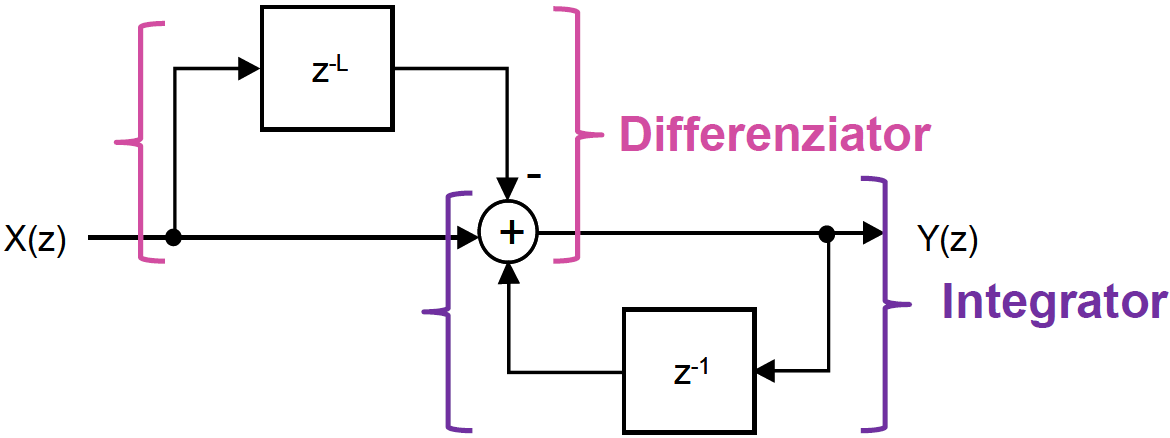
\includegraphics[width=\columnwidth]{images/kammfilter_IIR-filter.png}
\end{minipage}

\subsubsection*{Frequenzgang kaskadierte Kammfilter}

\begin{minipage}[c]{0.4\columnwidth}
    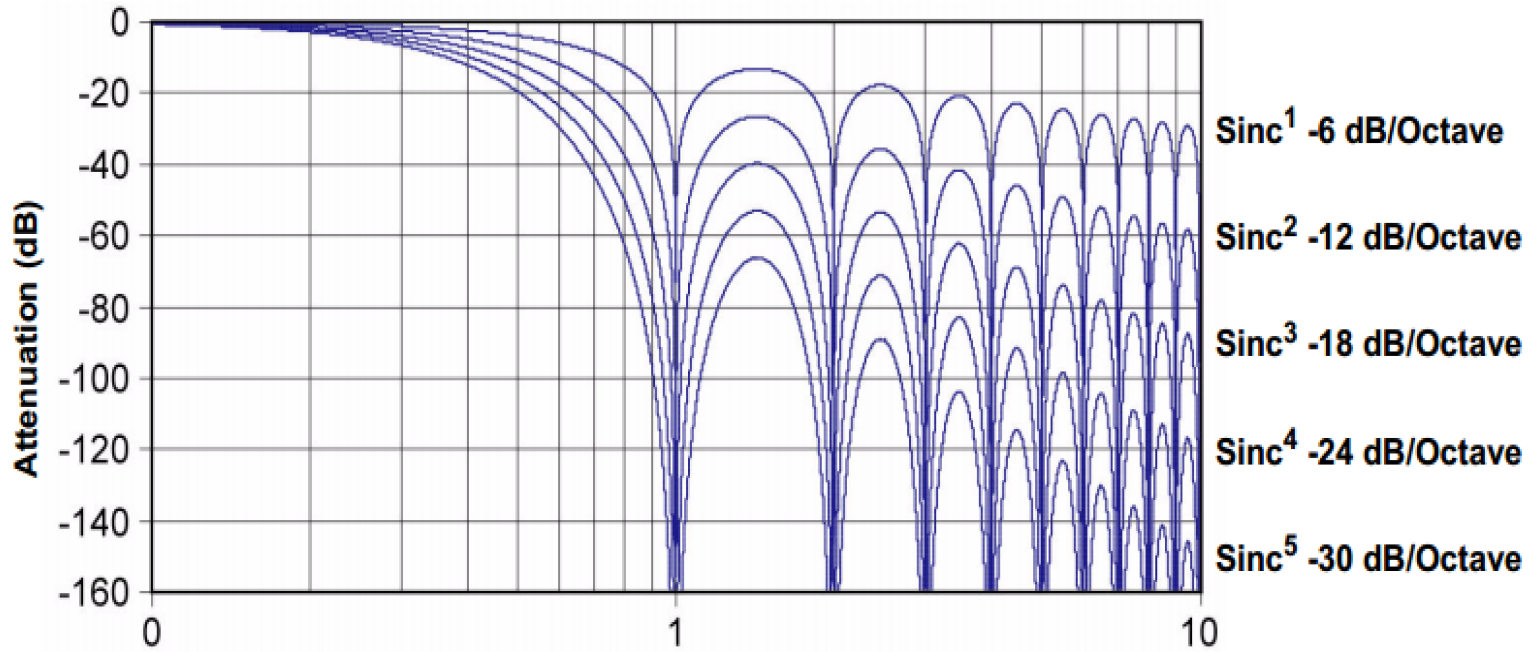
\includegraphics[width=\columnwidth]{images/frequenzgang_kaskadierte_kammfilter.png}
\end{minipage}
\hfill
\begin{minipage}[c]{0.58\columnwidth}
    \begin{itemize}
        \item Bezeichnung kaskadierte Kammfilter: \\
            CIC (Cascaded-Integrator-Comb-Filter)
        \item Notches ('Auslöschungen') bei $n \cdot \frac{\text{Sampling-Freq.}}{L}$
        \item Je höher die Ordnung, desto steiler der Abfall im Amplitudengang
    \end{itemize}
\end{minipage}

